\documentclass[12pt,a4paper,oneside]{article} % part, *section, *paragraph
%\documentclass[12pt,a4paper,oneside]{report} % part, *chapter, *section, *paragraph
%\documentclass[12pt,a4paper,oneside]{book} % part, *chapter, *section, *paragraph

\usepackage[english]{babel}
\usepackage[latin2]{inputenc}
\usepackage{setspace}
\usepackage{float}
\usepackage[T1]{fontenc} %\showhyphens{integetnem} \showhyphens{meggy�ltetv�ny}
%\usepackage{ucs}\usepackage[utf8x]{inputenc}
%\usepackage{fullpage} %\usepackage[margin=2cm]{geometry}
%\usepackage{amsmath,amssymb}
\usepackage{url} %VAGY %\usepackage[unicode]{hyperref}
\usepackage{listings}
%\usepackage{color} 
\usepackage{graphicx}
\usepackage{times}
\usepackage{fullpage}
%\usepackage{showkeys} % \label{} ki�r�sa \ref{}hez
 
\let\stdsection\section
\renewcommand\section{\clearpage\stdsection}
\begin{document}
\onehalfspacing
\begin{center}
\vspace{2em}
%\large{\bf{}BUDAPESTI M\H{U}SZAKI \'ES GAZDAS\'AGTUDOM\'ANYI EGYETEM}
\vspace{.5em}

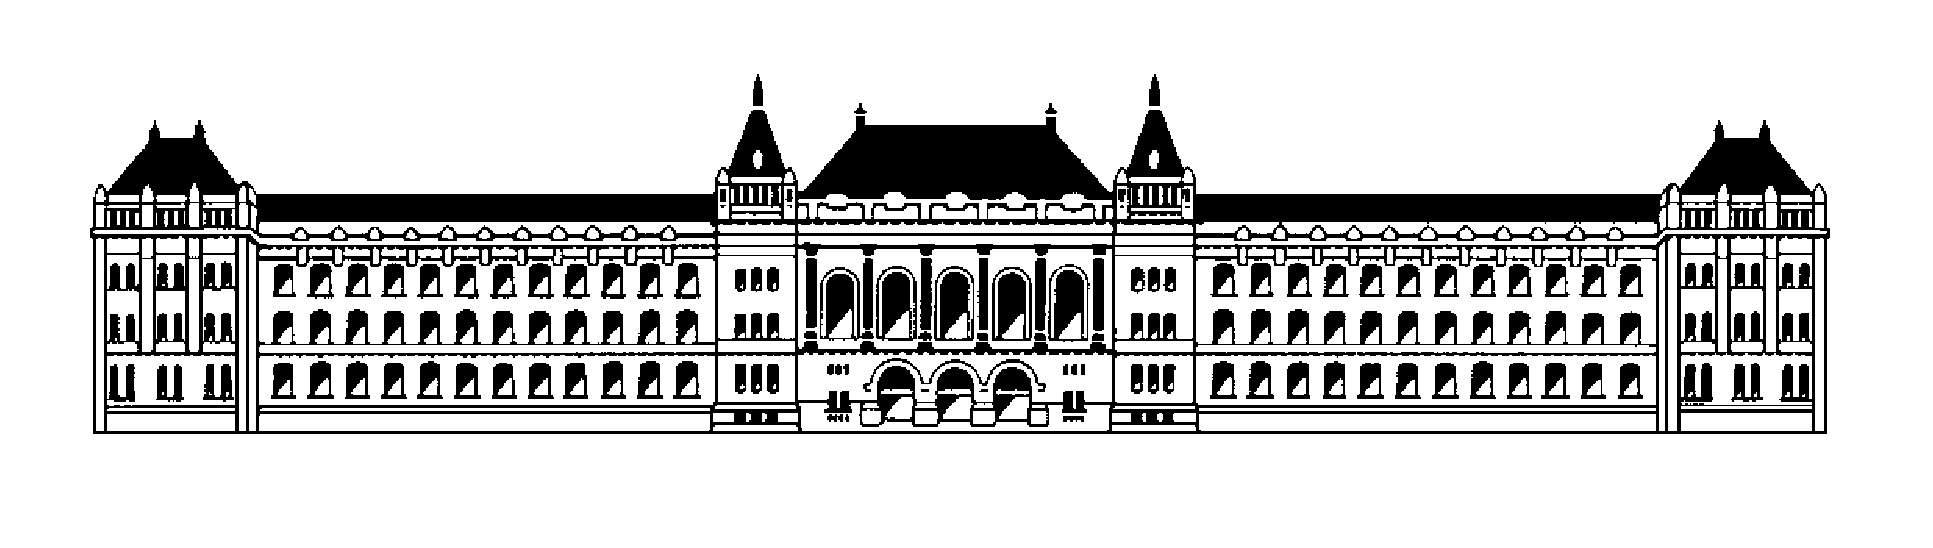
\includegraphics[width=60mm]{10000000000004C00000014A5D3CE278.eps}

Budapest University of Technology and Economics

Department of Measurement and Information Systems
%\vspace{.5em}

%\large{\bf{}VILLAMOSM\'ERN\"OKI \'ES INFORMATIKAI KAR\\
%M\'ERN\"OK INFORMATIKUS SZAK}

\vspace{2em}

%\Large{Informatikai Technol\'ogi\'ak szakir\'any\\
%Rendszerfejleszt\'es \'agazat}

%\vspace{1.5em}

%\Large{\bf{}\"On\'all\'o labor (BMEVIIIA337)}

%\vspace{1.5em}

\LARGE{\bf{}RTF tokenizer for LibreOffice writerfilter (rewrite of the RTF import)}

\vspace{2em}

\begin{tabular}{ l c}
  %hopefully i can avoid the photo this time
  %\parbox{30mm}{\includegraphics[width=20mm]{20090926.eps}} &
  \parbox{120mm}{
\begin{center}
\normalsize{Vajna Mikl�s (AYU9RZ),

4th semester, (MSc) computer engineering student

Consultants: C�dric Bosdonnat, M�t� Andr�s, Novell

Internal consultant: Horv�th �kos, MIT

Specialization in Dependable System Design

Internship Report

2011/12. 1st semester}
\end{center}
} \\
\end{tabular}


\end{center}
\thispagestyle{empty}
\newpage

\tableofcontents
\newpage

\section{Introduction}

LibreOffice\cite{libreoffice}.

\section{Background}

Bla bla.


\section{Design}

Bla bla.

\section{Implementation}

Bla bla.

\section{Testing}

Bla bla.

\section{Future work}

Bla bla.

\clearpage

\begin{thebibliography}{4}
\addcontentsline{toc}{section}{References}

\bibitem{libreoffice} Libreoffice, http://libreoffice.org/

\end{thebibliography}

\end{document}
